
% Infrastruktur
% Implementierung
	% Ordnerstruktur
	% Patterns
		% PageObject
		% PageFactory
	% Architektur
		% TestRunners
	% Testbeschreibung

\chapter{Umsetzung}
\label{sec:umsetzung}

\section{Prozess}
Der Prozess wurde equivalent aufgesetzt, wie es im \cref{sec:konzept:prozess} \nameref{sec:konzept:prozess} beschrieben wurde.

\begin{figure}[H]
	\centering
	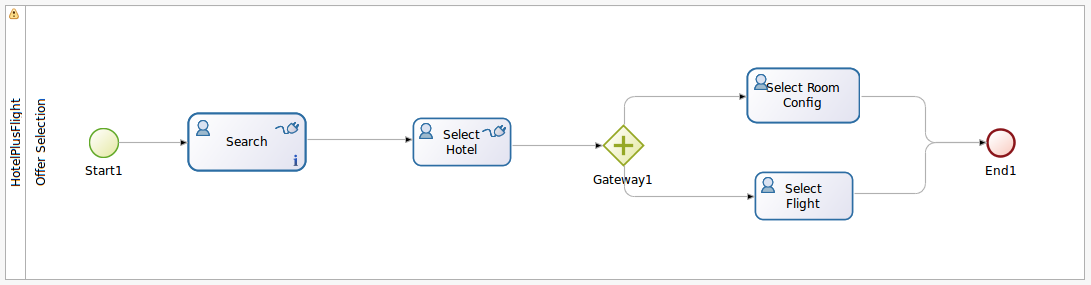
\includegraphics[width=1\textwidth]{images/umsetzung-prozess.png}
	\caption{Prozess im Bonita}
	\label{fig:umsetzung:prozess}
\end{figure}
Das Icon oben Links in den Task signalisiert, dass es sich dabei um einen Human Task handelt und eine Benutzerinteraktion erforderlich ist. Das Bild oben rechts in den Task zeigt an, dass es einen Connector auf dem Task gibt.

\section{Business Data Models und Pool Variables}
Als \glspl{bdm} wurden folgende Modelle definiert:
\begin{table}[H] 
	\caption{Business Data Models}
	\centering
	\label{sec:umsetzung:bdm:bdm}
	
	\begin{tabular}{ | l | l | c | } 
		\hline
		\textbf{Name} & \textbf{Type} & \textbf{Multiple} \\ \hline 
		\multicolumn{3}{|c|}{\textbf{HotelPlusFlightSearch}} \\ \hline 
		destination & string & \\ \hline
		departure & string & \\ \hline
		adults & integer & \\ \hline
		fromDate & date & \\ \hline
		toDate & date & \\ \hline
		id & string & \\ \hline
		\multicolumn{3}{|c|}{\textbf{HotelPlusFlightResults}} \\ \hline 
		hotels & HotelPlusFlightResultHotel & x \\ \hline
		\multicolumn{3}{|c|}{\textbf{HotelPlusFlightResultHotel}} \\ \hline 
		name & string & \\ \hline
		price & string & \\ \hline
		image & string & \\ \hline
		roomConfigs & HotelPlusFlightRoomConfig & x \\ \hline
		flights & HotelPlusFlightFlightResult & x \\ \hline
		id & string & \\ \hline
		\multicolumn{3}{|c|}{\textbf{HotelPlusFlightRoomConfig}} \\ \hline 
		roomType & string & \\ \hline
		mealType & string & \\ \hline
		id & string & \\ \hline
		\multicolumn{3}{|c|}{\textbf{HotelPlusFlightFlightResult}} \\ \hline 
		airline & string & \\ \hline
		fromAirport & string & \\ \hline
		toAirport & string & \\ \hline
		flight1FromTime & string & \\ \hline
		flight1ToTime & string & \\ \hline
		flight2FromTime & string & \\ \hline
		flight2ToTime & string & \\ \hline
		id & string & \\ \hline
	\end{tabular} 
\end{table}

Auf der Poolebene wurde für jedes \gls{bdm} eine Pool Variable erstellt. Der Name der Variable entspricht dem \gls{bdm}, beginnt jedoch mit einem kleinen Buchstaben.
\begin{table}[H] 
	\caption{Pool Variables}
	\centering
	\label{sec:umsetzung:bdm:poolvariable}
	
	\begin{tabular}{ | l | l | c | } 
		\hline
		\textbf{Name} & \textbf{BDM} \\ \hline 
		hotelPlusFlightSearch & HotelPlusFlightSearch \\ \hline
		hotelPlusFlightResults & HotelPlusFlightResults \\ \hline
		hotelPlusFlightResultHotel & HotelPlusFlightResultHotel \\ \hline
		hotelPlusFlightRoomConfig & HotelPlusFlightRoomConfig \\ \hline
	 	hotelPlusFlightFlightResult & HotelPlusFlightFlightResult \\ \hline
	\end{tabular} 
\end{table}
\section{Forms}
Die Formulare wurden bereits für die Mockups im \cref{sec:konzept:mockups} \nameref{sec:konzept:mockups} erstellt und konnten gleich wiederverwendet werden. Deshalb wird hier auf eine erneute Aufliestung verzichtet.

\section{Connectors}
Nachfolgend werden die Definitionen und Implementationen der Connectors beschrieben. Zusätzlich werden für deren Ausführung weitere Abhängigkeiten benötigt, welche in Bonita definiert werden müssen.

\subsection{Abhängigkeiten}
Für die Ausführung der Connectoren können in Bonita weitere Libraries hinterlegt werden. Für dieses Projekt wurde zusätzlich zwei Abhängigkeiten definiert. Zum einen Gson\footcite{Gson_2016-06-12}, für die Bearbeitung von JSON, and Handy URI Templates\footcite{HandyUriTempaltes_2016-06-12}, für die Verarbeitug von URI Templates gemäss RFC 6570\footcite{RFC_6570_-_URI_Template_2016-06-21}

\subsection{Definitions}
Es wurden vier Definitionen erstellt, für jeden Task einen.

\begin{table}[H] 
	\caption{Connector Definitions}
	\centering
	\label{sec:umsetzung:connectors:definitions}
	
	\begin{tabular}{ | l | l | l | l | } 
		\hline
		\textbf{Name} & \textbf{Input} & \textbf{Wizard pages} & \textbf{Outputs} \\ \hline 
		H+FSearch & H+FSearch & & H+FResults \\ \hline
		H+FResultsHotelSelection & HotelPlusFlightResults & Results & H+FResultHotel \\ \hline
		H+FHotelConfiguration & H+FResultHotel & Hotel & H+FResults \\ \hline
		H+FFlightSelection & H+FResultHotel & Hotel & H+FFlightResult \\ \hline
	\end{tabular} 
\end{table}

\subsection{Implementations}

\section{Tasks}
Nachfolgend werden die Tasks im Prozess beschrieben. Diese bestehen aus einem Bezeichner und einem Connector. Zusätzlich müssen noch der Contract, das Formular sowie die Operations (siehe \cref{sec:analyse:bonita:forms} \nameref{sec:analyse:bonita:forms}) angegeben werden.

\subsection{Search}
Der Search Task muss ein Formular darstellen damit der Benutzer seine Suchkriterien eingeben kann. Dazu wird der Connector HotelPlusFlugSearch hinterlegt und das Formular hotelPlusFlightSearchForm unter Connectors out definiert.

Folgender Contract und Operations mussten spezifiziert werden:
\begin{table}[H] 
	\caption{Search Task Contract}
	\centering
	
	\begin{tabular}{ | l | l | c | } 
		\hline
		\textbf{Name} & \textbf{Type} & \textbf{Multiple} \\ \hline 
		hotelPlusFlightSearchInput & complex & \\ \hline
		\hspace*{5mm}destination & text & \\ \hline
		\hspace*{5mm}departure & text & \\ \hline
		\hspace*{5mm}adults & integer & \\ \hline
		\hspace*{5mm}fromDate & date & \\ \hline
		\hspace*{5mm}toDate & date & \\ \hline
	\end{tabular} 
\end{table}
\begin{table}[H] 
	\caption{Search Task Operations}
	\centering
	
	\begin{tabular}{ | l | l | l | } 
		\hline
		\textbf{Business Data Model} & \textbf{Operation} & \textbf{Form Variable} \\ \hline 
		hotelPlusFlightSearch & setDestination & H+FSearchInput.destination \\ \hline
		hotelPlusFlightSearch & setDeparture & H+FSearchInput.departure \\ \hline
		hotelPlusFlightSearch & setAdults & H+FSearchInput.adults \\ \hline
		hotelPlusFlightSearch & setFromDate & H+FSearchInput.fromDate \\ \hline
		hotelPlusFlightSearch & setToDate & H+FSearchInput.toDate \\ \hline
	\end{tabular} 
\end{table}

\subsection{Select Hotel}
Der Select Hotel Task nimmt eine Liste von Hotels entgegen und speichert danach das selektierte ab. Dazu wird der Connector HotelPlusFlightResultsHotelSelection unter Connectors out und das Formular hotelPlusFlightHotelSelection hinterlegt.

Folgender Contract und Operations mussten spezifiziert werden:
\begin{table}[H] 
	\caption{Select Hotel Task Contract}
	\centering
	
	\begin{tabular}{ | l | l | c | } 
		\hline
		\textbf{Name} & \textbf{Type} & \textbf{Multiple} \\ \hline 
		hotelPlusFlightResultsInput & complex & \\ \hline
		\hspace*{5mm}hotels & complex & x \\ \hline
		\hspace*{10mm}name & text & \\ \hline
		\hspace*{10mm}price & text & \\ \hline
		\hspace*{10mm}image & text & \\ \hline
	\end{tabular} 
\end{table}
\begin{table}[H] 
	\caption{Select Hotel Task Operations}
	\centering
	
	\begin{tabular}{ | l | l | l | } 
		\hline
		\textbf{Business Data Model} & \textbf{Operation} & \textbf{Form Variable} \\ \hline 
		hotelPlusFlightSearch & setDestination & H+FSearchInput.destination \\ \hline
		hotelPlusFlightSearch & setDeparture & H+FSearchInput.departure \\ \hline
		hotelPlusFlightSearch & setAdults & H+FSearchInput.adults \\ \hline
		hotelPlusFlightSearch & setFromDate & H+FSearchInput.fromDate \\ \hline
		hotelPlusFlightSearch & setToDate & H+FSearchInput.toDate \\ \hline
	\end{tabular} 
\end{table}

\subsection{Select Room Config}
Beim Schritt Select Room Config wird das selektierte Hotel übergeben und der Benutzer kann eine Zimmer konfiguration auswählen. Dafür ist das From hotelPlusFlightSelectRoomConfig und der Connector HotelPlusFlightHotelConfiguration (im Connector out) vorgesehen.

Folgender Contract und Operations mussten spezifiziert werden:
\begin{table}[H] 
	\caption{Select Room Config Task Contract}
	\centering
	
	\begin{tabular}{ | l | l | c | } 
		\hline
		\textbf{Name} & \textbf{Type} & \textbf{Multiple} \\ \hline 
		hotelPlusFlightRoomConfigsInput & complex & \\ \hline
		\hspace*{5mm}configs & complex & x \\ \hline
		\hspace*{10mm}RoomType & text & \\ \hline
		\hspace*{10mm}MealType & text & \\ \hline
		\hspace*{10mm}Price & text & \\ \hline
	\end{tabular} 
\end{table}
\begin{table}[H] 
	\caption{Select Room Config Task Operations}
	\centering
	
	\begin{tabular}{ | l | l | l | } 
		\hline
		\textbf{Business Data Model} & \textbf{Operation} & \textbf{Form Variable} \\ \hline 
		hotelPlusFlightRoomConfig & setConfig & H+FRoomConfigsInput.config \\ \hline
	\end{tabular} 
\end{table}

\subsection{Select Flight}
Beim letzten Task muss der User ein Flug auswählen. Dazu wird dem Task das gewählte Hotel übergeben. Definiert wurde das Formular hotelPlusFlightSelectFlight und der Connector out HotelPlusFlightFlightSelection.

Folgender Contract und Operations mussten spezifiziert werden:
\begin{table}[H] 
	\caption{Select Flight Task Contract}
	\centering
	
	\begin{tabular}{ | l | l | c | } 
		\hline
		\textbf{Name} & \textbf{Type} & \textbf{Multiple} \\ \hline 
		hotelPlusFlightFlightResultsInput & complex & \\ \hline
		\hspace*{5mm}flights & complex & x \\ \hline
		\hspace*{10mm}Airline & text & \\ \hline
		\hspace*{10mm}FromAirport & text & \\ \hline
		\hspace*{10mm}ToAirport & text & \\ \hline
		\hspace*{10mm}Flight1FromTime & text & \\ \hline
		\hspace*{10mm}Flight1ToTime & text & \\ \hline
		\hspace*{10mm}Flight2FromTime & text & \\ \hline
		\hspace*{10mm}Flight2ToTime & text & \\ \hline
	\end{tabular} 
\end{table}
\begin{table}[H] 
	\caption{Select Flight Task Operations}
	\centering
	
	\begin{tabular}{ | l | l | l | } 
		\hline
		\textbf{Business Data Model} & \textbf{Operation} & \textbf{Form Variable} \\ \hline 
		hotelPlusFlightFlightResult & setFlight & H+FFlightsInput.flight \\ \hline
	\end{tabular} 
\end{table}